\documentclass[aspectratio=169]{beamer}

%\includeonlyframes{current}

\usepackage[utf8]{inputenc}
\usepackage[american]{babel}
\usepackage{amsmath,amsthm}
\usepackage{unicode}
\usepackage{array,tabularx}
\usepackage{ifthen}
\usepackage{tikz}
\usetikzlibrary{calc,arrows,arrows.meta,intersections}
\usepackage{tikzsymbols}

%\usepackage{ulem}

\mode<presentation>{%
  \usetheme{ibm}
}

\newcommand{\C}{ℂ}
\newcommand{\R}{ℝ}
\newcommand{\Z}{ℤ}
\newcommand{\N}{ℕ}
\newcommand{\Q}{ℚ}
\newcommand{\F}{\mathbb{F}}
\renewcommand{\P}{\mathbb{P}}
\renewcommand{\O}{\mathcal{O}}
\newcommand{\tildO}{\mathcal{\tilde{O}}}
\newcommand{\poly}{\operatorname{poly}}
\newcommand{\polylog}{\operatorname{polylog}}
\newcommand{\End}{\operatorname{End}}
\newcommand{\Hom}{\operatorname{Hom}}
\newcommand{\Cl}{\operatorname{Cl}}
\newcommand{\GL}{\operatorname{GL}}
\newcommand{\SL}{\operatorname{SL}}
\newcommand{\cyc}[1]{{〈 #1 〉}}
\newcommand{\sm}[2]{\left(\protect\begin{smallmatrix}#1\protect\\#2\protect\end{smallmatrix}\right)}

\renewcommand{\a}{\mathfrak{a}}
\renewcommand{\b}{\mathfrak{b}}
\newcommand{\g}{\mathfrak{g}}
\newcommand{\G}{\mathcal{G}}
\newcommand{\E}{\mathcal{E}}
\DeclareMathOperator{\rank}{rank}

\title{SQIsign}
\subtitle{past, present and future}
\author{Luca De Feo}
\date[April 28, 2025, The SQIparty]{April 28, 2025\\
  The SQIparty, Lleida, Spain}
\institute{IBM Research Zürich}

\begin{document}

\frame[plain]{\titlepage}

%%

\begin{frame}{What crypto from isogenies?}
  \small
  \renewcommand{\arraystretch}{1.5}
  \begin{tabular}{l p{0.25\textwidth} p{0.25\textwidth} p{0.25\textwidth}}
    & \emph{Key exchange / Encryption} & \emph{Identification / Signature} & \emph{Other}\\
    \hline
    \emph{Quadratic}
    & Couveignes--Rostovtsev--Stolbunov\par CSIDH\par SCALLOP
                                & SeaSign\par CSI-FiSh\par PEGASIS\footnote{See P. Dartois' talk on Wednesday.}
                                                             & Threshold\footnote{See G. Borin's talk on Tuesday.}\par PAKE\par \dots\\
    \emph{Quaternionic}
    & ---
                                & \strut\emph{SQIsign}\par SIDH-like signatures
                                                             & Ring signatures\par Adaptor signatures\par \dots\footnote{See I. Radulescu's talk on Tuesday.}\\
    \emph{\textit{Ad hoc}}
    & \strut\alert{SIDH~$\dagger$}\par SIDH fixes\par FESTA
                                & SIDH-like signatures
                                                             & Time-release crypto\par\dots
  \end{tabular}
\end{frame}

%%

\begin{frame}{Zero-Knowledge Proofs of Knowledge}
  \centering
  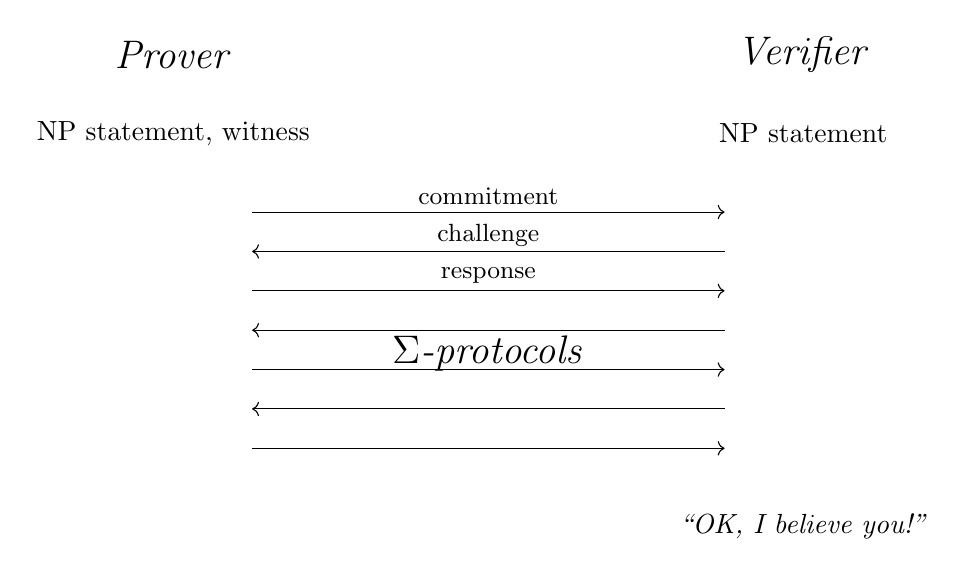
\begin{tikzpicture}
    \node at (0,0) {\Large\emph{Prover}};
    \node at (0,-1) {NP statement, witness};
    
    \node at (8,0) {\Large\emph{Verifier}};
    \node at (8,-1) {NP statement};

    \draw
    (1,-2) edge[->] +(6,0)
    ++(0,-0.5) edge[<-] +(6,0)
    ++(0,-0.5) edge[->] +(6,0);
    \uncover<1>{
      \draw
      (1,-3.5) edge[<-] +(6,0)
      ++(0,-0.5) edge[->] +(6,0)
      ++(0,-0.5) edge[<-] +(6,0)
      ++(0,-0.5) edge[->] +(6,0);
    }
      
    \node at (8, -6) {\textit{``OK, I believe you!''}};

    \uncover<2->{
      \draw
      (4,-1.8) node{\small commitment}
      ++(0,-0.5) node{\small challenge}
      ++(0,-0.5) node{\small response}
      ++(0,-1) node{\Large\emph{$\Sigma$-protocols}};
    }
  \end{tikzpicture}
\end{frame}

%%

\begin{frame}{Soundness: \textit{``I really know the secret''}}
  \begin{description}
    \setlength{\itemsep}{1em}
  \item[Minimal definition:]<1-> A prover with no knowledge of the secret
    only convinces the verifier with negligible probability.
  \item[Extractor:]<2-> An algorithm that \emph{extracts} the witness by
    interacting repeatedly with the prover.
  \end{description}

  \begin{uncoverenv}<2->
    \begin{center}
      \begin{tikzpicture}
        \node[anchor=west] at (0,0) {\emph{Extractor \uncover<3->{(2-special soundness)}}};
        \draw (0,0) to ++(0,-4) to ++(12,0) to ++(0,4) to ++(-6.8,0);
        \draw[->] (12,-3) to ++(1,0) node[anchor=west]{witness};
        
        \begin{scope}[shift={(.5,-.5)}]
          \small
          \node[anchor=north west] at (0,0) {\emph{Prover}};
          \draw (0.5,-1) edge[->] node[above] {\footnotesize commitment} +(4,0)
          ++(0,-.7) edge[<-,blue] node[above] {\footnotesize challenge} +(4,0)
          ++(0,-.7) edge[->,blue] node[above] {\footnotesize response} +(4,0);
          \draw[black] (0,0) -- ++(4,0) -- ++(0,-3) -- ++(-4,0) -- ++(0,3);
        \end{scope}

        \newcount\shift
        \animate<3-8>
        \animatevalue<3-8>{\shift}{0}{6}
        \begin{scope}[shift={(\the\shift + 0.5,-.5)}]
          \small
          \node[anchor=north west] at (0,0) {\emph{Prover}};
          \draw (0.5,-1) edge[->] node[above] {\footnotesize commitment} +(4,0);
          \uncover<8->{
            \draw (0.5,-1.7) edge[<-,purple] node[above] {\footnotesize challenge'} +(4,0)
            ++(0,-.7) edge[->,purple] node[above] {\footnotesize response'} +(4,0);
          }
          \draw[black] (0,0) -- ++(4,0) -- ++(0,-3) -- ++(-4,0) -- ++(0,3);
        \end{scope}
      \end{tikzpicture}
    \end{center}
  \end{uncoverenv}
\end{frame}

%%

\begin{frame}{Zero-Knowledge: \textit{``You learned nothing about the secret''}}
  \centering
  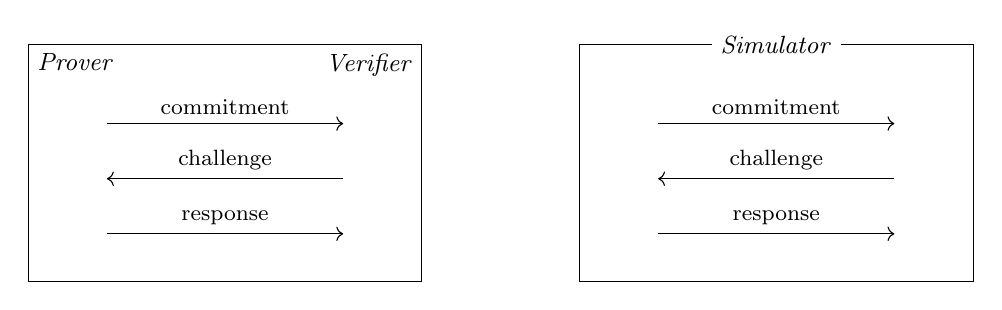
\begin{tikzpicture}
    \begin{scope}
      \small
      \node[anchor=north west] at (0,0) {\emph{Prover}};
      \node[anchor=north east] at (5,0) {\emph{Verifier}};
      \draw (1,-1) edge[->] node[above] {\footnotesize commitment} +(3,0)
      ++(0,-.7) edge[<-] node[above] {\footnotesize challenge} +(3,0)
      ++(0,-.7) edge[->] node[above] {\footnotesize response} +(3,0);
      \draw[black] (0,0) -- ++(5,0) -- ++(0,-3) -- ++(-5,0) -- ++(0,3);
    \end{scope}
    
    \begin{scope}[xshift=7cm]
      \small
      \draw (1,-1) edge[->] node[above] {\footnotesize commitment} +(3,0)
      ++(0,-.7) edge[<-] node[above] {\footnotesize challenge} +(3,0)
      ++(0,-.7) edge[->] node[above] {\footnotesize response} +(3,0);
      \draw[black] (0,0) -- ++(5,0) -- ++(0,-3) -- ++(-5,0) -- ++(0,3);
      \node[fill=white] at (2.5,0) {\emph{Simulator}};
    \end{scope}
  \end{tikzpicture}
\end{frame}

%%

\begin{frame}
  \centering
  \includegraphics[height=0.95\textheight]{ali-baba}
\end{frame}

%%

\begin{frame}{A ZK-PoK for Graph Isomorphism (after Goldwasser--Micali--Rackoff)}
  \centering
  \begin{tikzpicture}
    \begin{scope}
      \Large
      \node (G) at (0,0) {$G$};
      \node (H) at (4,0) {$H$};

      \draw[->] (G) edge node[above]{$\sigma$} (H);

      \uncover<2->{
        \node (R) at (2,-3) {$R$};
      }
      \uncover<2>{
        \draw[->] (G) edge node[left]{$\pi$} (R);
      }

      \uncover<4->{
        \draw[->,dashed] (R) edge node[right]{$\sigma\circ\pi^{-1}$} (H);
        \draw[->,dashed] (R) edge node[left]{$\pi^{-1}$} (G);
      }
    \end{scope}

    \draw[gray] (6,1) -- ++(0,-5);
    
    \begin{scope}[xshift=8cm]
      \node at (0,0) {\emph{Prover}};
      \node at (4,0) {\emph{Verifier}};

      \uncover<2->{
        \draw[->] (0,-1) to node[above]{$R$} ++(4,0);
      }

      \uncover<3->{
        \draw[<-] (0,-2) to node[above]{$b\in\{0,1\}$} ++(4,0);
      }

      \uncover<4->{
        \draw[->] (0,-3) to node[above]{$\sigma^b\circ\pi^{-1}$} ++(4,0);
      }
    \end{scope}
  \end{tikzpicture}
\end{frame}

%%

\begin{frame}{The ``Group Action'' point of view }
  \begin{columns}
    \begin{column}{0.5\textwidth}
      \centering
      \begin{tikzpicture}
        \Large
        \node (G) at (0,0) {$G$};
        \node (H) at (4,0) {$H$};

        \draw[->] (G) edge node[above]{$\sigma$} (H);
        \node (R) at (2,-3) {$R$};
        \draw[->,dashed] (R) edge node[left]{$\pi^{-1}$} (G);
        \draw[->,dashed] (R) edge node[right]{$\sigma\circ\pi^{-1}$} (H);
      \end{tikzpicture}  
    \end{column}
    \begin{column}{0.5\textwidth}
      \begin{itemize}
        \setlength{\itemsep}{2em}
      \item ``Public'' set: \emph{$G,H,R \in \mathcal{S}$}
      \item ``Private'' group: \emph{$\pi,\sigma \in \mathcal{G}$}
      \item Group action: \emph{$\mathcal{G} \circlearrowright \mathcal{S}$}
      \end{itemize}
    \end{column}
  \end{columns}
\end{frame}

%%

\begin{frame}{More on group actions}
  \begin{description}
  \item[Protocols:]\ 
    \begin{itemize}
    \item Giacomo Borin\\
      --- \textit{Threshold signatures from different group actions}
    \end{itemize}
  \item[Instantiations:]\
    \begin{itemize}
    \item Marc Houben\\
      --- \textit{A Montgomery-ladder for isogenies}
    \item Pierrick Dartois\\
      --- \textit{PEGASIS: Practical Effective Class Group Action
        using 4-Dimensional Isogenies}
    \item Eli Orvis\\
      --- \textit{Generalized class group actions via class field
        theory}
    \end{itemize}
  \end{description}
\end{frame}

%%

\begin{frame}{The birth of SQIsign}
  \centering
  \only<1>{
    \includegraphics[height=0.8\textheight]{seaside}
  }
  \only<2->{
    \includegraphics[width=\textwidth]{aussois-school}

    \bigskip

    \uncover<3->{
      \Large{the \emph{\huge S}hort \emph{\huge Q}uaternion and \emph{\huge I}sogeny \emph{\huge sign}ature}

      \bigskip
    
      {\footnotesize De Feo, Kohel, Leroux, Petit, Wesolowski --- Asiacrypt 2020}
    }
  }
\end{frame}

%%

\begin{frame}
  \Large
  \begin{tikzpicture}[remember picture,overlay,shift={(current page.center)},xscale=0.5]
    \fill[white] (0,8) -- (16,8) -- (16,-8) -- (0,-8);
    \fill[ibmblue] (0,8) -- (-16,8) -- (-16,-8) -- (0,-8);

    \draw[ibmblue]
    (8,3) node {Maximal order}
    ++(0,-2) node {Ideal}
    ++(0,-2) node {Ideal class}
    ++(0,-2) node {Norm};
    \draw[white]
    (-8,3) node {Endomorphism ring}
    ++(0,-2) node {Isogeny}
    ++(0,-2) node {$\Hom(E,E')$}
    ++(0,-2) node {Degree};

  \end{tikzpicture}
\end{frame}

%%

\begin{frame}{More on correspondences}
  \begin{description}
  \item[Algorithms for the Deuring correspondence:]\
    \begin{itemize}
    \item Jordi Pujolàs\\
      --- \textit{On prime degree twisting endomorphisms of
        supersingular elliptic curves}
    \end{itemize}
  \item[Higher dimensions:]\ 
    \begin{itemize}
    \item Enric Florit\\
      --- \textit{Quaternionic multiplication and abelian fourfolds}
    \item Péter Kutas\\
      --- \textit{Biquaternion cryptography}
    \end{itemize}
  \item[Other kinds:]\
    \begin{itemize}
    \item Harun Kir\\
      --- \textit{Exploring Kani's Research}
    \item Chloe Martindale\\
      --- \textit{Hidden geometry in supersingular isogeny graphs}
    \end{itemize}
  \end{description}
\end{frame}

%%

\begin{frame}{Propagating EndRing info}
  \centering
  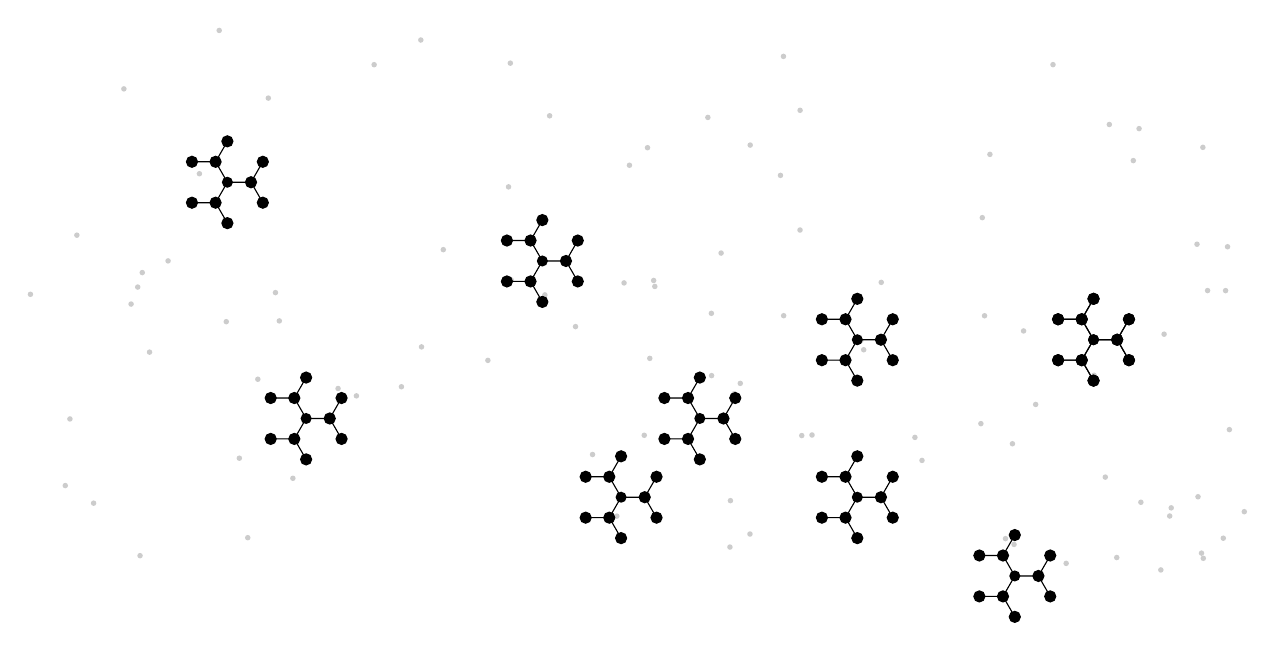
\begin{tikzpicture}
    \pgfmathsetseed{12345}
    \foreach \i in {1,...,100} {
      \pgfmathparse{16*random()}
      \let\x\pgfmathresult
      \pgfmathparse{7*random()}
      \let\y\pgfmathresult
      \fill[black!20!white] (\x,\y) circle (1pt);
    }
    \foreach \i in {1,...,10} {
      \pgfmathparse{floor(15*random())}
      \let\x\pgfmathresult
      \pgfmathparse{floor(6*random())}
      \let\y\pgfmathresult
      \fill (\x,\y) circle (2pt);
      \uncover<2->{
        \foreach \rho in {0,1,2} {
          \draw[fill,-latex] (\x,\y) -- +(120*\rho:.3) circle (2pt);
          \uncover<3->{
            \foreach \sigma in {-1,1} {
              \draw[fill,-latex] (\x,\y) ++(120*\rho:.3) -- ++(120*\rho+60*\sigma:.3) circle (2pt);
            }
          }
        }
      }
    }
  \end{tikzpicture}
\end{frame}

%%

\begin{frame}{SQIsign}
  \transdissolve<4,6>
  \large
  \centering
  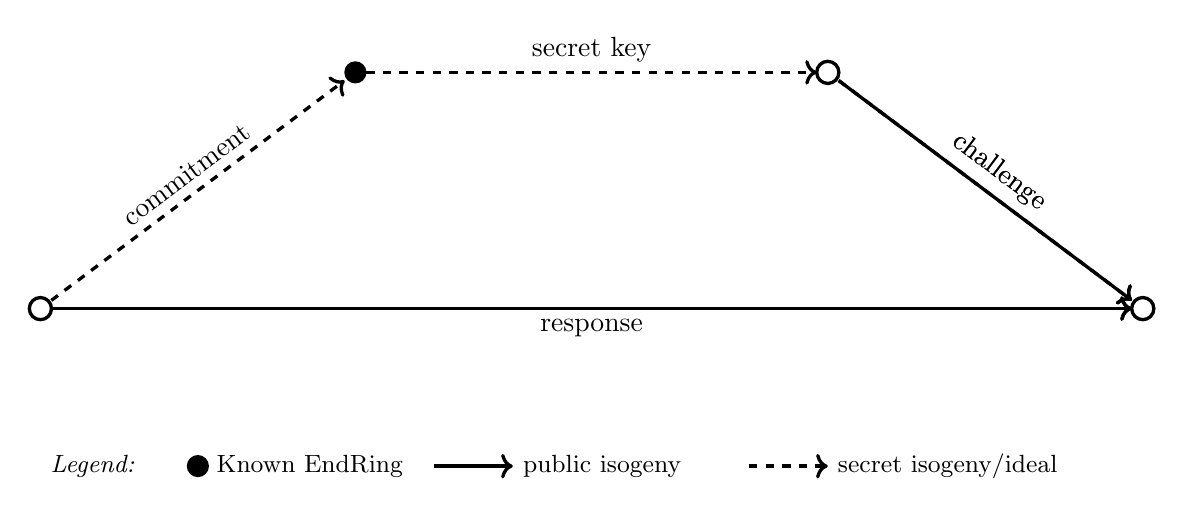
\begin{tikzpicture}[very thick]
    \fill
    (0,3) node(E0){} circle (4pt);
    \draw
    (6,3) node(PK){} circle (4pt);
    \draw[dashed,->] (E0) edge node[above,sloped] {secret key} (PK);
    
    \uncover<2->{
      \draw (-4,0) node(COM){} circle (4pt);
      \draw[dashed,->] (COM) edge node[sloped,above] {commitment} (E0);
    }

    \uncover<3->{
      \draw (10,0) node(CH){} circle (4pt);
    }
    \uncover<3,6->{
      \draw (PK) edge[->] node[sloped,above] {challenge} (CH);
    }

    \uncover<4-5>{
      \draw (PK) edge[dashed,->] node[sloped,above] {challenge} (CH);
    }

    \uncover<5>{
      \draw (COM) edge[dashed,->] (CH);
    }

    \uncover<6->{
      \draw (COM) edge[->] node[below] {response} (CH);
    }

    \begin{scope}[shift={(-4,-2)},anchor=west]
      \small
      \node at (0,0) {\emph{Legend:}};
      \fill (2,0) node(E0){~Known EndRing} circle (4pt);
      \draw[->] (5,0) to ++(1,0) node {public isogeny};
      \draw[->,dashed] (9,0) to ++(1,0) node {secret isogeny/ideal};
    \end{scope}
  \end{tikzpicture}
\end{frame}

%%

\begin{frame}{2-special soudness $\to$ OneEnd}
  \large
  \centering
  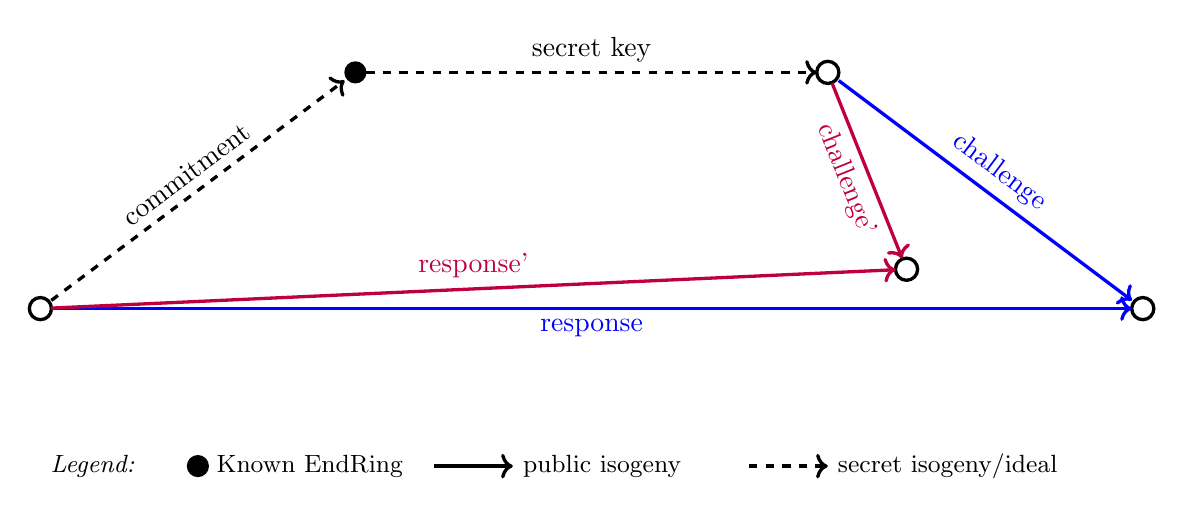
\begin{tikzpicture}[very thick]
    \fill (0,3) node(E0){} circle (4pt);
    \draw (6,3) node(PK){} circle (4pt);
    \draw (-4,0) node(COM){} circle (4pt);
    \draw (10,0) node(CH){} circle (4pt);
    
    \draw[dashed,->] (E0) edge node[above,sloped] {secret key} (PK);
    \draw[dashed,->] (COM) edge node[sloped,above] {commitment} (E0);
    \draw (PK) edge[blue,->] node[sloped,above] {challenge} (CH);
    \draw (COM) edge[blue,->] node[below] {response} (CH);

    \uncover<2->{
      \draw (7,0.5) node(CH1){} circle (4pt);
      \draw (PK) edge[purple,->] node[sloped,below] {challenge'} (CH1);
      \draw (COM) edge[purple,->] node[above] {response'} (CH1);
    }
    
    \begin{scope}[shift={(-4,-2)},anchor=west]
      \small
      \node at (0,0) {\emph{Legend:}};
      \fill (2,0) node(E0){~Known EndRing} circle (4pt);
      \draw[->] (5,0) to ++(1,0) node {public isogeny};
      \draw[->,dashed] (9,0) to ++(1,0) node {secret isogeny/ideal};
    \end{scope}
  \end{tikzpicture}
\end{frame}

%%

\begin{frame}{What response?}
  \large
  \centering
  \begin{tikzpicture}[very thick]
    \fill (0,3) node(E0){} circle (4pt);
    \draw (6,3) node(PK){} circle (4pt);
    \draw (-4,0) node(COM){} circle (4pt);
    \draw (10,0) node(CH){} circle (4pt);
    
    \draw[dashed,->] (E0) edge node[above,sloped] {secret key} (PK);
    \draw[dashed,->] (COM) edge node[sloped,above] {commitment} (E0);
    \draw (PK) edge[dashed,->] node[sloped,above] {challenge} (CH);
    \draw (COM) edge[dashed,->] node[below] {response} (CH);

    \node at (-4,-2) {};
  \end{tikzpicture}
\end{frame}

%%

\begin{frame}
  \begin{tikzpicture}[remember picture,overlay]
    \node at (current page.center) {\includegraphics[width=\paperwidth]{monoski}};
    \node[white,anchor=north west] at (current page.north west) {\Large SQIsigning like it's the 80s};
  \end{tikzpicture}
\end{frame}

%%

\begin{frame}{KLPT: translating quaternion ideals to smooth degree isogenies}
  \begin{block}{Kohel, Lauter, Petit, Tignol (2014)}
    \begin{description}
    \item[Input:] a left ideal class of a \alert{special} maximal order
    \item[Output:] a \alert{unique} representative of norm a power of 2
    \end{description}
  \end{block}
  
  \begin{block}{De Feo, Kohel, Leroux, Longa, Petit, Wesolowski (2020,2022)}
    \begin{description}
    \item[Input:] a left ideal class of an \alert{arbitrary} maximal order
    \item[Output:] a \alert{sort of random looking} representative of
      norm a power of 2
    \end{description}
  \end{block}
\end{frame}

%% 

\begin{frame}{Performance of SQIsign v1 \small(June 2023)}
  \begin{table}[h]
    \centering
    \begin{tabular}{ r r | r r r | c }
      \multicolumn{2}{c|}{Bytes} & \multicolumn{3}{c|}{Mcycles}\\
      Public Key & Signature & Keygen & Sign & Verify & Security \\
      \hline
       64 & 177 & 3,728 & 5,779 & 108 & NIST-1 \\
       96 & 263 & 23,734 & 43,760 & 654 & NIST-3 \\
      128 & 335 & 91,049 & 158,544 & 2,177 & NIST-5 \\
    \end{tabular}
  \end{table}
\end{frame}

%%

\begin{frame}{Zero-Knowledge}
  \centering
  \begin{tikzpicture}[scale=0.5]
    \small
    \begin{scope}
      \node[anchor=east] at (-6,1.5) {\emph{Real transcript:}};
      
      \fill (0,3) node(E0){} circle (4pt);
      \draw (6,3) node(PK){} circle (4pt);
      \draw (-4,0) node(COM){} circle (4pt);
      \draw (10,0) node(CH){} circle (4pt);
      \foreach \s in {1,...,9} {
        \fill ($(COM)!\s/10!(CH)$) circle (2pt);
      }
      \foreach \s in {1,...,4} {
        \fill ($(PK)!\s/5!(CH)$) circle (2pt);
      }
      
      \draw[dashed,->] (E0) edge node[above,sloped] {secret key} (PK);
      \draw[dashed,->] (COM) edge node[sloped,above] {commitment} (E0);
      \draw (PK) edge[->] node[sloped,above] {challenge} (CH);
      \draw (COM) edge[->] node[below] {response} (CH);
    \end{scope}

    \begin{scope}[yshift=-8cm]
      \node[anchor=east] at (-6,1.5) {\emph{Simulated transcript:}};

      \fill (0,3) node(E0){} circle (4pt);
      \draw (6,3) node(PK){} circle (4pt);
      
      \uncover<2->{
        \draw (10,0) node(CH){} circle (4pt);
        \draw (PK) edge[->] (CH);
        \foreach \s in {1,...,4} {
          \fill ($(PK)!\s/5!(CH)$) circle (2pt);
        }
      }
      \uncover<3->{
        \draw (-4,0) node(COM){} circle (4pt);
        \draw (COM) edge[->] (CH);
        \foreach \s in {1,...,9} {
          \fill ($(COM)!\s/10!(CH)$) circle (2pt);
        }
      }
    \end{scope}
  \end{tikzpicture}  
\end{frame}

%%

\begin{frame}
  \begin{tikzpicture}[remember picture,overlay]
    \node at (current page.center) {\includegraphics[width=\paperwidth]{ski-jump}};
    \node[anchor=north west] at (current page.north west) {\Large Modern SQIsigning};
  \end{tikzpicture}
\end{frame}

%%

\begin{frame}{SQIsignHD (Dartois, Leroux, Robert, Wesolowski 2023)}
  \begin{columns}
    \begin{column}{0.5\textwidth}
      \centering
      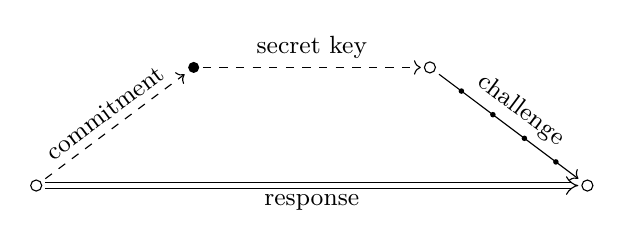
\begin{tikzpicture}[scale=0.5]
        \small
        \begin{scope}
          \fill (0,3) node(E0){} circle (4pt);
          \draw (6,3) node(PK){} circle (4pt);
          \draw (-4,0) node(COM){} circle (4pt);
          \draw (10,0) node(CH){} circle (4pt);
          \foreach \s in {1,...,4} {
            \fill ($(PK)!\s/5!(CH)$) circle (2pt);
          }
          
          \draw[dashed,->] (E0) edge node[above,sloped] {secret key} (PK);
          \draw[dashed,->] (COM) edge node[sloped,above] {commitment} (E0);
          \draw (PK) edge[->] node[sloped,above] {challenge} (CH);
          \draw (COM) edge[double distance=2pt,-Implies] node[below] {response} (CH);
        \end{scope}
      \end{tikzpicture}  
    \end{column}
    \begin{column}{0.5\textwidth}
      \begin{itemize}
        \setlength{\itemsep}{2em}
      \item Response encoded by interpolation points,
      \item Evaluate using 4D isogeny formulas,
      \item \emph{$++$ Fast signing,}
      \item \emph{$++$ Shorter responses,}
      \item \alert{$--$ Slow verification.}
      \end{itemize}
    \end{column}
  \end{columns}
\end{frame}

%%

\begin{frame}{SQIsign2D {\footnotesize(Basso, Dartois, De Feo, Leroux, Maino, Nakagawa, Onuki, Pope, Robert, Wesolowski 2024)}}
  \begin{itemize}
    \setlength{\itemsep}{2em}
  \item Move from 4D to 2D isogeny representations.
  \item \emph{$++$ Fast signing,}
  \item \emph{$++$ Shorter responses,}
  \item \emph{$++$ Fast verification.}
  \end{itemize}
\end{frame}

%%

\begin{frame}{More on higher-dimensional isogenies}
  \begin{description}
  \item[Translating ideals to isogenies]\
    \begin{itemize}
    \item Jonathan Komada Eriksen\\
      --- \textit{Translating ideals to isogenies}
    \end{itemize}
  \item[Theta structures and isogenies:]\
    \begin{itemize}
    \item Maria Corte-Real Santos\\
      --- \textit{Computing two-dimensional isogenies for SQIsign}
    \item Max Duparc\\
      --- \textit{A Combinatorial Perspective on Theta Structures}
    \item Antoine Dequay\\
      --- \textit{Algorithms for moduli space of abelian varieties with level structure}
    \end{itemize}
  \item[More variants of SQIsign:]\
    \begin{itemize}
    \item Hiroshi Onuki\\
      --- \textit{SQIsign2DPush}
    \end{itemize}
  \end{description}
\end{frame}

%%

\begin{frame}{Other topics}
  \begin{description}
  \item[Better pairing computations:]\
    \begin{itemize}
    \item Alessandro Sferlazza\\
      --- \textit{Montgomery ladders already compute pairings}
    \end{itemize}
  \item[Abstracting SQIsign for cryptography:]\
    \begin{itemize}
    \item Ilinca Radulescu\\
      --- \textit{Cryptographic Categories}
    \end{itemize}
  \end{description}
\end{frame}

%%

\begin{frame}{Performance of SQIsign v2 \small(February 2025)}
  \begin{table}[h]
    \centering
    \begin{tabular}{ r r | r r r | c }
      \multicolumn{2}{c|}{Bytes} & \multicolumn{3}{c|}{Mcycles}\\
      Public Key & Signature & Keygen & Sign & Verify & Security \\
      \hline
      66 & 148 & 84 & 203 & 11 & NIST-1 \\
      98 & 222 & 228 & 549 & 31 & NIST-3 \\
      130 & 294 & 403 & 1021 & 62 & NIST-5 \\
    \end{tabular}
  \end{table}

  \bigskip
  \emph{More on performance and platform-specific implementations:}
  \begin{itemize}
  \item Benjamin Smith\\
    --- \textit{Post-quantum signatures in practice: securing IoT software updates}
  \item Décio Gazzoni Filho\\
    --- \textit{Speeding up SQIsign verification on the ARM Cortex-M4}
  \end{itemize}
\end{frame}

%%

\begin{frame}{Zero-knowledge}
  \begin{columns}
    \begin{column}{0.5\textwidth}
      \centering
      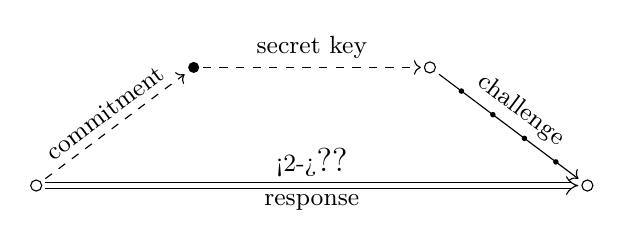
\begin{tikzpicture}[scale=0.5]
        \small
        \begin{scope}
          \fill (0,3) node(E0){} circle (4pt);
          \draw (6,3) node(PK){} circle (4pt);
          \draw (-4,0) node(COM){} circle (4pt);
          \draw (10,0) node(CH){} circle (4pt);
          \foreach \s in {1,...,4} {
            \fill ($(PK)!\s/5!(CH)$) circle (2pt);
          }

          \uncover<1>{
            \draw[dashed,->] (E0) edge node[above,sloped] {secret key} (PK);
            \draw[dashed,->] (COM) edge node[sloped,above] {commitment} (E0);
          }
          \draw (PK) edge[->] node[sloped,above] {challenge} (CH);
          \draw (COM) edge[double distance=2pt,-Implies]
          node[below] {response}
          node[above] {\only<2->{\large\alert{??}}} (CH);
        \end{scope}
      \end{tikzpicture}
    \end{column}
    \begin{column}{0.5\textwidth}
      \begin{itemize}
        \setlength{\itemsep}{1em}
      \item HD response encoded by interpolation points
      \item<2-> How to evaluate large degree isogenies without EndRing?
      \item<2-> \textit{Ad-hoc} fix: give a magic box to simulator.
      \item<3-> Recent progress: Aardal, Basso, De Feo, Patranabis,
        Wesolowski (eprint 2025/379)
      \end{itemize}
    \end{column}
  \end{columns}
\end{frame}

%%

\begin{frame}{The future}
  \begin{columns}
    \begin{column}{0.5\textwidth}
      \begin{description}
      \item[Todos:]\
        \begin{itemize}
        \item Systematic analysis of variants
        \item Hardware accelerations
        \end{itemize}
      \item[Challenges:]\
        \begin{itemize}
        \item Better security proof
        \item Constant time algorithms
        \item SQIsign needs stability
        \end{itemize}
      \end{description}
    \end{column}
    \begin{column}{0.5\textwidth}
      \begin{description}
      \item[Looks tough:]\
        \begin{itemize}
        \item Meaningfully faster signatures
        \end{itemize}
      \item[One may always dream:]\
        \begin{itemize}
        \item Meaningfully faster verification
        \item Better 1D SQIsign
        \end{itemize}
      \end{description}
    \end{column}
  \end{columns}
\end{frame}

\end{document}


% LocalWords:  Isogeny abelian isogenies hyperelliptic supersingular Frobenius
% LocalWords:  isogenous
